
% Bosch Latex Vorlage 
% !TeX root = ../Inhalt_alles/Vorlage.tex
% Diese Vorlage soll vor allem einen Header bieten, der für die meisten Laborberichte und Arbeiten sinnvoll ist und hoffentlich einige nützliche Dinge in LaTeX zeigt.
% Bisher ist sie von Steffen Brahtz und Thomas Lübbehüsen gepflegt worden, gerne können aber Sachen von anderen ergänzt werden.
\documentclass[
12pt,
a4paper,
headings=small,                    % Überschriften etwas kleiner, Geschmackssache
bibliography=totoc,                % Bibliography-Kapitel im Inhaltsverzeichnis anzeigen
listof=totoc,                      % Listof-Kapitel im Inhaltsverzeichnis anzeigen
parskip=half*,                     % Nur halbe Einzüge vor erste Zeile eines Absatzes, stattdessen Abstand zwischen Absätzen
]{scrartcl}                        % Artikel-Klasse (die simpleste) mit KOMA-Skripten (die können ein paar Sachen mehr als Latex nur so)
% Für größere Sachen (Studienarbeit, Teamprojekt, BA) empfiehlt sich scrrprt statt scrartcl

%%%%%%%%%%%%%%%%%%%%%% Bitte Ausfüllen %%%%%%%%%%%%%%%%%%%%%%%%%%%%%%
\newcommand{\myAuthorA}{Max Mustermann}
\newcommand{\AutorAMartikelnummer}{012 345 67}
\newcommand{\myAuthorB}{Moni Musterfrau} % Einfach leerlassen, wenn es keinen zweiten gibt
\newcommand{\AutorBMartikelnummer}{012 345 67} % Einfach leerlassen, wenn es keinen zweiten gibt
\newcommand{\myGroup}{Gruppe X00}
\newcommand{\myTitle}{Versuch X}

%%%%%%%%%%%%%%%%%%%%%%% für titelseite anpassen sonst egal %%%%%%%%%%%%%%%
\newcommand{\myFakultaet}{Elektrotechnik}
\newcommand{\myTextArt}{Dokumentation zum Teamprojekt} % auch für sperrvermerk gültig
\newcommand{\myStudiengang}{Elektro- und Informationstechnik im Praxisverbund}
\newcommand{\myPruefer}{Prof. Dr. Rainer Bermbach}
\newcommand{\einreichDatum}{DD.MM.YYYY}
\newcommand{\textUeberOstfaliaBox}{$ $} % zusätzlicher text über der frabigen box
\newcommand{\strasseFackultaet}{Salzdahlumer Str. 46/48} % änderen wenn man oben im campus ist 

%%%%%%%%%%%%%%%%%%%%%%%% für Erklärung anpassen %%%%%%%%%%%%%%%%%%%%%%%%%%%%%%%%%%%%
\newcommand{\myOrt}{Hildesheim}
%%%%%%%%%%%%%%%%%%%%%%%%% Standardpakete %%%%%%%%%%%%%%%%%%%%%%%%%
\usepackage[utf8]{inputenc}        % Eingabe von Umlauten im Code
\usepackage[T1]{fontenc}           % Enkodierung von Output, böse Dinge passieren ohne dieses Package
\usepackage[ngerman]{babel}        % Deutsches Sprachpaket
\usepackage{scrhack}               % Fixt Probelem mit KOMA-Skript
\usepackage{mathtools}             % Mathematische Formeln
\usepackage{microtype}             % Macht irgendwie typographisch besseren Text
\usepackage{graphicx}              % Hinzufügen von Bildern / PDFs über \includegraphics{bildname}
\usepackage{caption}               % Erweiterte Captions für Bilder, Formeln, ...
\usepackage{physics}               % Zusätzliche wissenschaftliche Symbole und Differentialquotient mit \dd{...}
\usepackage{hyperref}              % Links und Verweise in PDFs
\usepackage{siunitx}               % Wissenschaftlich korrektes Angeben von Zahlen / Einheiten (wichtig bei Hampe, Siaenen), u.A. Einheiten nicht kursiv
\usepackage{listings}              % Includen von Code
\usepackage{xcolor}                % Einfach eigene Farben definen
\usepackage{url}                   % Includenb von Links mit \url{http://thomas-harriehausen.de}             

%%%%%%%%%%%%%%%%%%%%%%%%% Optionale Pakete, die auch entfernt werden können %%%%%%%%%%%%%%%%%%%%%%%%%
\usepackage{lastpage}              % Erlaubt "Seite 2 von x" im Footer, da es die Anzahl Seiten ausgibt
\usepackage{float}                 % Welches dann in Kombination mit [H] auch wirklich die Gleitumgebung mit dem Bild oder der Tabelle an die richtige Stelle packt, nämlich (H)ere 
\usepackage{array}                 % Matrizen in Latex
\usepackage{tabularx}              % Tabellen, die advanced sind
\usepackage{enumitem}              % Erweiterte Aufzählungen, bespielsweise alternative Aufzählungssymbole 
\usepackage{gensymb}               % Für Grad-Symbol \degree, Ohm: \ohm und einige mehr
\usepackage{esvect}                % Vektorpfeile mittels \vv{E}
\usepackage{icomma}                % Richtgen Abstand beim Dezimaltrennzeichen
\usepackage[all]{nowidow}          % Vermeidet "widows" (einzelne Zeilen auf nächster Seite die noch zum Absatz gehören)
\usepackage{chngcntr}              % Ermöglicht Ändern von Nummerierung (Formeln, Bilder), z.B. Zählen innerhalb Kapitel
\usepackage{subcaption}            % Bilder nebeneinander darstellen
\usepackage{csquotes}              % Für Zitate und um Warnung von babel zu unterdrücken
\usepackage[draft]{todonotes}      % \todo[inline]{beispiel}-Befehl, der Kommentare hinzufügt. Ausblenden der Todos durch ersetzen von "draft" durch "disable"
\usepackage{multirow}              % Für Tabellen: Mehrere Zeilen in einer Spalte miteinander verbinden
\usepackage{booktabs}              % Für das Excel2LaTeX-Addon, s.u. in Tipps
\usepackage{bigstrut}              % Für das Excel2LaTeX-Addon, s.u. in Tipps
\usepackage{cancel}                % Für durchgestrichenen Text (schlechte Messwerte zB) mit \cancel{text}
\usepackage{easyfig}               % Einfaches includen von Bildern z.B.: \Figure[caption={LOL}, width=\textwidth]{dateiname} (Labels sind automatisch \autoref{fig:dateiname})
\usepackage{tcolorbox}             % Für colorboxes (genutzt für Titelseite)
\usepackage{pgfplots}              % Um Diagramme direkt mit Latex zu erstellen
\usepackage{xifthen}               % Für if else Logic, wird im Header benutzt
\usepackage{pdfpages}              % Um PDF Dokument hinzuzufügen
\usepackage{makecell}			   % ermögtlicht einfache Zeilenumbrüche in einer tabelle
%%%%%%%%%%%%%%%%%%%%%%%%% Einstellung für Pakete und LaTeX %%%%%%%%%%%%%%%%%%%%%%%%%
% Bestimmte Warnung von chktex (Latex linter) deaktivieren:
% chktex-file 46
% chktex-file 2
% chktex-file 1
% chktex-file 41
% chktex-file 10
% chktex-file 17

% Language Tool in vs code auf deutsch stellen (Extension LTex installieren):
%LTeX: language=de-DE

% Einstellen von Seitenabständen und Größen
\usepackage[paper=a4paper, 
left=25mm,                    
right=20mm,                   
top=15mm,                     
bottom=15mm,                  
includehead,includefoot            % Fuß- und Kopfzeile berücksichtigen
]{geometry}

% Schriftart ändern
\usepackage[space]{erewhon} % Main Schriftart 1 
%\usepackage{stix2} % Main Schriftart 2
\usepackage{tgheros} % Serifenlose Schriftart, wird deshalb nur für Überschriften genutzt
%\usepackage[stix2,vvarbb]{newtxmath} % Nur sinnvoll wenn aktiverte Schrifart keine (schönen) Math-Symbole hat
% Optional: Serifenlose Schriftart aktivieren um Leute zu triggern
%\renewcommand{\familydefault}{\sfdefault}

\setcounter{secnumdepth}{6} % tiefere referenz ebene möglich z.b. paragraph \label{key}

% Automatisch Text wie "Zitat" in deutsche Anführungszeichen umwandeln
\MakeOuterQuote{"}

% Warnung von pgfplot unterdrücken
\pgfplotsset{compat=1.7}

% Einstelllungen für das siuntix-Paket
\sisetup{
	per-mode=fraction,             % Einheiten als Brüche statt ^-1
	locale=DE,                     % Malpunkt, statt Kreuz
	output-decimal-marker={,},     % Komma als Dezimaltrennzeichen
	group-digits=true,             % Zifferngruppierung an/aus (in 3er Blöcken)
	group-separator=\text{~},      % Abstand als Trennzeichen für Zifferngruppierung
	group-minimum-digits=5,        % Ziffern ab minimal 5 Ziffern gesamt gruppieren
	detect-all,                    % Benutze gleiche Schriftarten wie im Text
	range-phrase=--,               % Komma in Range
	range-units=single,             % Nur einmal die Einheit bei Range
	exponent-to-prefix = true,	% bei eingabe von \SI{1.7e3}{\g} kommt 1,7 kg raus 
	%	exponent-to-prefix = false,		% bei eingabe von \SI{1.7e3}{\g} kommt 1,7\cdot 10^3 g raus 	
	%	scientific-notation = engineering, % nimmt die exponenten nach der Ingienuerschreibwese ! Achtung bei der S umgebung der Tablle mit table-format !
	scientific-notation = false,
	output-complex-root = j,		 % anstelle i j ausgeben
	complex-root-position = before-number, % stellt das j vor der zahl
	exponent-product = \cdot
} 

%Die Umgebung von TableS is gleich zu Table, allerdings wird scientific-notation ausgeschaltet innerhalb der Umgebung. Falls Fehler wie: "Package siunitx Error: No space reserved for an exponent" immer tableS statt table verwenden!
\newenvironment{tableS}{\sisetup{scientific-notation = false}  \begin{table}}{\end{table}\sisetup{scientific-notation = engineering} }
                                 
\DeclareSIUnit\divisor{div.}       % SIunitx: Volt pro Divisor, zB bei Schirmbildern      
\DeclareSIUnit\voltpeak{Vp}        % Für Vp in SI
\DeclareSIUnit\voltppeak{Vpp}      % Für Vpp in SI    

% Biblatex includen für Zitieren
\usepackage[style=numeric,         % Zitieren mit [1] statt [Ein05]
sorting=none,                      % Referenzen sotieren nach Ort des Auftauchen
backend=bibtex                     % Unterdrückt irgendeine Warnung
]{biblatex} 
%\addbibresource{../sources.bib}       % Optional, fügt sources.bib aus gleichem Verzeichnis hinzu
%\addbibresource{../../sources.bib}       % Optional, fügt sources.bib aus gleichem Verzeichnis hinzu
\setcounter{biburllcpenalty}{7000} % für lange URLs im Quellverzeichnis
\setcounter{biburlucpenalty}{8000} %

% Hinzufügen von Fuß- und Kopfzeilen mit Trennlinie
\usepackage[
headsepline,
footsepline,
automark
]{scrlayer-scrpage}   

% circutikz-Paket: "Zeichnen" von Schaltungen im Code
\usepackage[european,              % Europäischer Style für ciruitikz
straightvoltages,                  % Gerade Zählpfeile in DE
americaninductors,                 % Meist wird alte Norm mit Ami-Spulen genutzt
siunitx,                           % Integration von siunitx aktivieren
nooldvoltagedirection              % Neue Art für Spannungsrichtung
]{circuitikz}                      

% Quellen ab x starten
%\newcommand{\quellenstart}{3} 
%\DeclareFieldFormat{labelnumber}{
%    \ifinteger{#1}
%    {\number\numexpr#1+\quellenstart\relax}
%    {#1}}

% Zählen innerhalb von Kapitel für Bilder / Gleichungen: <section>.<number>
\counterwithin{figure}{section}
\counterwithin{table}{section}
\counterwithin{equation}{section}

% Bilder in diesen Subfoldern müssen den Folder beim includen nicht mehr im Dateinamen angeben
\graphicspath{{../fig/}{../bilder/}{../Bilder/}{../images/}{../figs/}{../../fig/}{../../bilder/}{../../Bilder/}{../../images/}{../../figs/}}

% Höherer Zeilenabstand, Dirty Harrie will eigentlich 1.2, ist außerdem gut, weil's nach mehr Seiten aussieht
\linespread{1.15}

% Latex sorgt dafür, dass linebreaks stärker erzwungen werden und nicht Wörter über den Rand hinausragen; siehe https://texfaq.org/FAQ-overfull
\tolerance=7500
\pretolerance=200

% Etwas mehr Abstand zwischen den einzelnen aligns
\addtolength{\jot}{0.4em}

% Macht vertikalen Abstand in Tabellen größer, dieser ist default sehr eng
\renewcommand{\arraystretch}{1.15} 

% Kein Einschub bei Auflistungen, Geschmackssache
\setlist[enumerate]{leftmargin=*}

% Aufzählungen mit a) b) statt 1. 2.
\renewcommand{\labelenumi}{\alph{enumi})}

% Ersetzt alle * im Math-Environment durch richtige Malzeichen (cdot). Wenn * für konj. komplex oder ähnliches genutzt werden soll, dann auskommentieren
%\mathcode`\*="8000
%{\catcode`\*\active\gdef*{\cdot}}

% Indizes standardmäßig NICHT kursiv, da es nach DIN-Norm eher in Ausnahmen kursiv ist. Hilfreich für MET- und EMT-Labor ausnahme mit \mathit{}
% bsp : \mathit{A_X}  -> Ausgabe ist A kursiv indizi X nicht kursiv 
\makeatletter
\begingroup
\catcode`\_=\active
\protected\gdef_{\@ifnextchar|\subtextit\subtextup }
\endgroup
\def\subtextit|#1|{\sb{#1}}
\def\subtextup#1{\sb{\mathrm{#1}}}
\AtBeginDocument{\catcode`\_=12 \mathcode`\_=32768}
\makeatother

% Gleichung in Formel umbennen, Harrie mag das lieber
\renewcommand{\equationautorefname}{Formel} %% not working

% Für das todonotes package
\reversemarginpar                  % Randnotizen auf der linken Seite, da dort mehr Platz ist
\setlength{\marginparwidth}{2cm}   % Randnotizen-Breite festlegen, da das Paket sonst nicht funktioniert 

% Einige vordefinierte Colors
\definecolor{listingbg}{cmyk}{0,0,0,0.05}
\definecolor{ostfalia-magenta}{cmyk}{0,1,0,0}
\definecolor{ostfalia-green}{cmyk}{0.3,0,1,0}
\definecolor{ostfalia-cyan}{cmyk}{0.78,0,0.32,0}
\definecolor{ostfalia-orange}{cmyk}{0,0.3,1,0}
\definecolor{ostfalia-yellow}{cmyk}{0,0.05,1,0}
\definecolor{ostfalia-violet}{cmyk}{0.86,0.96,0,0}
\definecolor{ostfalia-wf-blue}{cmyk}{1,0,0,0}
\definecolor{ostfalia-blue}{cmyk}{1,0.75,0,0.3}

% Eigenes Aussehen für Code-Blöcke definieren, kopiert von 
% https://github.com/Wandmalfarbe/pandoc-latex-template
\definecolor{listing-background}{HTML}{F7F7F7}
\definecolor{listing-rule}{HTML}{B3B2B3}
\definecolor{listing-numbers}{HTML}{B3B2B3}
\definecolor{listing-text-color}{HTML}{000000}
\definecolor{listing-keyword}{HTML}{435489}
\definecolor{listing-keyword-2}{HTML}{1284CA} % additional keywords
\definecolor{listing-keyword-3}{HTML}{9137CB} % additional keywords
\definecolor{listing-identifier}{HTML}{435489}
\definecolor{listing-string}{HTML}{00999A}
\definecolor{listing-comment}{HTML}{8E8E8E}

%%%%%%%%%%%%%%%%%%%%%%%%% Eigene Befehle %%%%%%%%%%%%%%%%%%%%%%%%%
% Kleines Underline, was sich gut für komplexe Zahlen eignet, z.B. \ul{U}_q
\newcommand{\ul}[1]{\underline{#1\mkern-1.5mu}\mkern 1.5mu}
% Text hervorheben als code / mono
\newcommand{\code}[1]{\ttfamily#1\rmfamily} % Beispiel: \code{AC}-Modus
% \desc{} Command für Text in Math-Mode mit Abstand vor und nach dem Text, nützlich um zB in align etwas beschreiben. z.B.: \desc{eingesetzt ergibt dies:}
\newcommand{\desc}[1]{{\hspace*{0,7 cm}\text{#1}\hspace*{0,7 cm}}}

\newcommand{\paraNumOFF}{
	\renewcommand{\theparagraph}{\thesection.\arabic{subsection}.\arabic{subsubsection} \alph{paragraph})}
} % aufzählung im paragraph mit 1.1.2 a). 1.1.2 b). und 1.1.2 c).

\newcommand{\paraNumON}{
	\renewcommand{\theparagraph}{\thesection.\arabic{subsection}.\arabic{subsubsection}.\arabic{paragraph}}
} % aufzählung bei paragraph mit 1.1.2.1 1.2.2 und 1.1.2.3


\newcommand{\subsubSecNumOFF}{
	\renewcommand{\thesubsubsection}{\thesection.\arabic{subsection} \alph{subsubsection})}
} % aufzählung im subsubsectionmit 1.1 a). 1.1 b). und 1.1 c).

\newcommand{\subsubSecNumON}{
	\renewcommand{\thesubsubsection}{\thesection.\arabic{subsection}.\arabic{subsubsection}}
} % aufzählung bei subsubsectionmit 1.1.1 1.2.2 und 1.1.3


% Buchstaben vor Subsections für Laborberichte (V2.2, A3.1, usw.) Benutzung mit \laborsubsection{V}{Überschriftstext}
\newcommand{\laborsubsection}[2] {
	\renewcommand{\thesubsection}{#1 \thesection.\arabic{subsection}}
	\subsection{#2}
	\renewcommand{\thesubsection}{\thesection.\arabic{subsection}}
}
% Einfacher Befehl, um Subsection wieder bei 1 starten, damit Wechsel von V 2.2 zu D 2.1 möglich ist
\newcommand{\resetlaborsectioncounter}{\setcounter{subsection}{0}}

% Helfer-Makro, wird weiter unten im Header benutzt.
\newcommand{\ifempty}[3]{\ifthenelse{\equal{#1}{}}{#2}{#3}}

% Abkürzungen mit korrekten Typographie (achtung Autismus)
\newcommand*{\zb}{z.\,B.~\allowbreak}
\newcommand*{\ua}{u.\,a.~\allowbreak}

%Euler Form (e^j)
\newcommand{\keulerg}[2][]{\mathrm{e}^{\mathrm{#1j}\,#2^\circ}} % komplexe zahl in euler form mit grad
\newcommand{\keulerk}[2][]{\mathrm{e}^{\mathrm{#1j}\,\left( #2\right) }} % komplexe zahl in euler form ohne grad mit klammern
\newcommand{\keuler}[2][]{\mathrm{e}^{\mathrm{#1j}\,#2}} % komplexe zahl in euler form ohne grad ohne klammern 
\newcommand{\dreiVec}[3]{\left( \begin{matrix}
		#1\\
		#2 \\
		#3 \\
	\end{matrix}\right) } % einfacher 3er vector mit einem Befehl \dreiVec{1}{2}{3} !nur in mathe umgebnungen ! 

\newcommand{\fancypara}[2][0.5ex]{\paragraph{{\boldmath #2 }} $ $ \\[#1]}   % pragraph welcher alles dick schreibt und man den Abstand zur neuen Zeile einstellen kann (standart abstand ist 0.5em).
\newcommand{\dummyLorem}{
Lorem ipsum dolor sit amet, consectetur adipiscing elit. Quisque nec consectetur lorem. Aliquam diam nisi, vestibulum et eleifend mollis, luctus sit amet diam. Donec in magna non enim lobortis ultricies eget ac eros. Etiam eget enim pretium arcu sagittis porttitor ac eu tellus. Curabitur quis cursus lorem. Aliquam auctor est auctor metus lobortis convallis. Maecenas elementum sem sed sem suscipit, a mattis justo volutpat. Praesent et pharetra ex. Morbi ac eros quam. Nullam id libero sit amet dolor aliquet tincidunt. Suspendisse scelerisque eleifend tristique. Curabitur nec nisi id arcu tempus malesuada vehicula at enim. } %dumm text
\newcommand{\dummy}{
	Text Text Text Text\\
	Text Text Text Text\\
	Text Text Text Text\\} 
% Eigene Daten, werden dann in PDF übernommen
\newcommand{\myAuthor}{\myAuthorA, \AutorAMartikelnummer} 
\newcommand{\mySecondAuthor}{\myAuthorB, \AutorBMartikelnummer}
\newcommand{\myDate}{\today} % \today kann durch Text ersetzt werden

 % header_teil1.tex ausgelagert, damit dies in Inkscape addon Tex Text genutzt werden kann
	\lstdefinestyle{eisvogel_listing_style}{
	language         = java,
	numbers          = left,
	xleftmargin      = 2.7em,
	framexleftmargin = 2.5em,
	backgroundcolor  = \color{listing-background},
	basicstyle       = \color{listing-text-color}\linespread{1.0}\small\ttfamily{},
	breaklines       = true,
	frame            = single,
	framesep         = 0.19em,
	rulecolor        = \color{listing-rule},
	frameround       = ffff,
	tabsize          = 4,
	numberstyle      = \color{listing-numbers},
	aboveskip        = 1.0em,
	belowskip        = 0.1em,
	abovecaptionskip = 0em,
	belowcaptionskip = 1.0em,
	keywordstyle     = {\color{listing-keyword}\bfseries},
	keywordstyle     = {[2]\color{listing-keyword-2}\bfseries},
	keywordstyle     = {[3]\color{listing-keyword-3}\bfseries\itshape},
	sensitive        = true,
	identifierstyle  = \color{listing-identifier},
	commentstyle     = \color{listing-comment},
	stringstyle      = \color{listing-string},
	showstringspaces = false,
	escapeinside     = {/*@}{@*/}, % Allow LaTeX inside these special comments
	literate         =
	{á}{{\'a}}1 {é}{{\'e}}1 {í}{{\'i}}1 {ó}{{\'o}}1 {ú}{{\'u}}1
	{Á}{{\'A}}1 {É}{{\'E}}1 {Í}{{\'I}}1 {Ó}{{\'O}}1 {Ú}{{\'U}}1
	{à}{{\`a}}1 {è}{{\'e}}1 {ì}{{\`i}}1 {ò}{{\`o}}1 {ù}{{\`u}}1
	{À}{{\`A}}1 {È}{{\'E}}1 {Ì}{{\`I}}1 {Ò}{{\`O}}1 {Ù}{{\`U}}1
	{ä}{{\"a}}1 {ë}{{\"e}}1 {ï}{{\"i}}1 {ö}{{\"o}}1 {ü}{{\"u}}1
	{Ä}{{\"A}}1 {Ë}{{\"E}}1 {Ï}{{\"I}}1 {Ö}{{\"O}}1 {Ü}{{\"U}}1
	{â}{{\^a}}1 {ê}{{\^e}}1 {î}{{\^i}}1 {ô}{{\^o}}1 {û}{{\^u}}1
	{Â}{{\^A}}1 {Ê}{{\^E}}1 {Î}{{\^I}}1 {Ô}{{\^O}}1 {Û}{{\^U}}1
	{œ}{{\oe}}1 {Œ}{{\OE}}1 {æ}{{\ae}}1 {Æ}{{\AE}}1 {ß}{{\ss}}1
	{ç}{{\c c}}1 {Ç}{{\c C}}1 {ø}{{\o}}1 {å}{{\r a}}1 {Å}{{\r A}}1
	{€}{{\EUR}}1 {£}{{\pounds}}1 {«}{{\guillemotleft}}1
	{»}{{\guillemotright}}1 {ñ}{{\~n}}1 {Ñ}{{\~N}}1 {¿}{{?`}}1
	{…}{{\ldots}}1 {≥}{{>=}}1 {≤}{{<=}}1 {„}{{\glqq}}1 {“}{{\grqq}}1
	{”}{{''}}1
}
\lstset{style=eisvogel_listing_style}
	% Header und Footer setzen mit KOMA
\clearpairofpagestyles{}
\ihead{\ifempty{\myAuthorB}{\myAuthorA, \AutorAMartikelnummer}{\myAuthorA, \AutorAMartikelnummer \\ \myAuthorB, \AutorBMartikelnummer}} % Erkennt automatisch die Anzahl der Autoren
\chead{\myGroup}
\ohead{\myTitle}
\ifoot{\myDate}
\ofoot{Seite \thepage{} von \pageref*{LastPage}}
%\automark{section} % Automatisch die aktuelle Section im Header anzeigen

% Metadaten ins generierte PDF
\hypersetup{
	pdftitle={\myTitle},
	pdfauthor={\myAuthorA{ mit der Matrikelnummer: }\AutorAMartikelnummer{, } \myAuthorB{ mit der Matrikelnummer: }\AutorBMartikelnummer },
	colorlinks=true, % Links farbig darstellen. Diese Zeile entfernen, um stattdessen roten Kästen um Links zu erzeugen, welche dann nicht gedruckt werden.
	allcolors=black % Farbe der Links einstellen
} % header_teil2.tex ausgelagert, damit header_teil1.tex in Inkscape addon Tex Text genutzt werden kann

%%%%%%%%%%%%%%%%%%%%%%%%% Tipps für TexStudio %%%%%%%%%%%%%%%%%%%%%%%%%
% Bessere Rechtschreibkorrektur in TexStudio hinzufügen: https://tex.stackexchange.com/a/282571/148289
% Tabellen-Autoformatierung mit dem blauen Button oben rechts in Tex-Studio
% Mehrere Zeilen gleichzeitig Bearbeiten mit gedrücktem STRG und Ziehen nach unten
% Word zu Latex Converter: https://www.docx2latex.com/ (Falls der Laborpartner zu inkompetent ist)
% Latex-Addin für Excel zum Exportieren von Tabellen, sehr gut: https://github.com/krlmlr/Excel2LaTeX/releases/latest (ZIP runterladen, extrahieren und einmal die xla-Datei ausführen)
% Excel-Addin zum (Batch-)Exportieren von Diagrammen als PNG, auch sehr gut: https://www.xltoolbox.net/de/
% Wenn VS Code genutzt wird, sollten die Addons Latex Workshop und LTeX installiert werden
%%%%%%%%%%%%%%%%%%%%%%%%% Tipps für Behele: %%%%%%%%%%%%%%%%%%%%%%%%%%%%

%Mulitplikation ohne Malzeichen:
%\, -> halbes Leerzeichen

%Zahlen in Euler Form (e^j):
%\keulerg[-]{150} -> e^-j150°
%\keulerg{150} -> e^j150°
%\keulerk[-]{150^\circ-20^\circ} -> e^-j(150°-20°)
%\keuler[-]{\left( 150^\circ-20^\circ\right) } -> e^-j(150°-20°) Klammern nicht automatisch

%Zahlen in kartesicher Form:
%\SI{8,854 + i4,865}{\volt} -> (8,854 + j4,865)V
%\num{2 + i3} -> 2 + j3

%Komplexe Zahlen
%\ul{I}_{12} -> I wird unterstrichen und 12 als Indizeh

%Einheiten
%\si{\farad} -> F (kleines si verarbeitet nur die Einheit)
%\SI{8,854}{\micro\farad} -> 8,854μF
%SI{20e-6}{\farad} -> 20*10^-6F

%Platzhalter für fehlendes Bild:
%\begin{figure}[H]
%	\centering
%	\missingfigure{TEXT ZUR BESCHREIBUNG WAS FEHLT}
%	\captionof{figure}{BILDUNTERSCHRIFT}
%	\label{fig:LABEL}
%\end{figure}

%Auf Kapitel, Gleichungen oder Bilder verweisen:
%Dem zu verweisenden Objekt ein label geben mit \label{NAME}
%Mittels \autoref{NAME} darauf verweisen

%Tabelle zu Latex
%https://tableconvert.com/?output=latex

%PDF Dokument einbinden
%\includepdf{"NAME DES PDFs"} 

\begin{document}
	\counterwithin{lstlisting}{section} % Muss leider hier stehen und kann nicht in den Header
	
	%% !TeX root = Vorlage.tex

\newgeometry{inner=2.5cm, outer=2.5cm, vmargin=2cm}

    
\begin{titlepage}
    \setlength{\parskip}{0cm}
    \setlength{\parindent}{0cm}
    \sffamily
    \begin{minipage}[t]{66mm}
        
\includegraphics[height=14mm]{figs/ostfalia_logo}\par
        \hfill%
        \begin{minipage}[t]{49mm}
            \color{ostfalia-wf-blue}\hrule height 1pt
            \vspace{0.5\baselineskip}
            Fakultät Elektrotechnik
        \end{minipage}
    \end{minipage}
        
    \vfill
    
    {\color[gray]{0.66}\hrule height 1pt}\vspace{0.5\baselineskip}
    
    {\large
        % ANPASSEN
        \myAuthorA \\
        \myAuthorB
    \par}\vspace{2\baselineskip}
    
    {\Huge
        % ANPASSEN
        \myTitle
    \par}\vspace{2\baselineskip}
    
    {\large
        % ANPASSEN
        Dokumentation zum Teamprojekt\\
        im Studiengang Elektroinformationstechnik im Praxisverbund\\
    \par}
    {\color[gray]{0.66}\hrule height 1pt}\vspace{4\baselineskip}

    {\large
        % ANPASSEN
        Prüfer:\\
        Prof. Dr. Rainer Bermbach\\[1\baselineskip]
        Eingereicht am DD.MM.YYYY
    \par}

    \vfill
    
    \begin{tcolorbox}[size=tight,
        oversize,
        sharp corners,
        colback=ostfalia-blue,
        colframe=ostfalia-blue,
        boxsep=2ex]
        \color{white}
        \textbf{Ostfalia Hochschule für angewandte Wissenschaften}\\
        -- Hochschule Braunschweig/Wolfenbüttel \textbullet~Salzdahlumer Str. 46/48 \textbullet~38302 Wolfenbüttel
    \end{tcolorbox}
    
\end{titlepage}

\restoregeometry % Optionale Titlepage titlepage.tex modifizieren 
	
	% Sperrvermerk für Studienarbeit/Teamprojekt/BA...
	%\input{../Zusatz/sperrvermerk_erklaerung
	
	
	
	
	%\includepdf{"NAME DES DECKBLATTS"} 
	
	
	
	\tableofcontents
	\newpage
	%%%%%%%%%%%%%%%%%%%%%%%%%%%%%%%%%%%%%%%%%%%%%%%%%%%%%%%%%%%%%%%%%%%%%%%%%%%%%%%
	%%%%%%%%%%%%%%%%%%%%%%%%%%%%%%%%%%%%%%%%%%%%%%%%%%%%%%%%%%%%%%%%%%%%%%%%%%%%%%%
	%%%%%%%%%%%%%%%%%%%%% Ab hier Text %%%%%%%%%%%%%%%%%%%%%%%%%%%%%%%%%%%%%%%%%%%%
	%%%%%%%%%%%%%%%%%%%%%%%%%%%%%%%%%%%%%%%%%%%%%%%%%%%%%%%%%%%%%%%%%%%%%%%%%%%%%%%
	%%%%%%%%%%%%%%%%%%%%%%%%%%%%%%%%%%%%%%%%%%%%%%%%%%%%%%%%%%%%%%%%%%%%%%%%%%%%%%%
	{\LARGE Nur Inhalt2}
	% um seins alleine (ohne labels des anderen) zuarbeiten ein % davor weg 
% standart einstellung ist alleine arbeiten 
%!TeX root = Vorlage_nur_inhalt1.tex
% um das gesammte dokuemnt zu erstellen oder um die labels des anderen zu nutzen einmalig ein % wegmachen und nach dem man fertig ist wieder ein % zeichen davor und bei der zeile darüber ein % weg sodass %!... steht
%% !TeX root = ../Inhalt_1+2/Vorlage.tex
%a%!TEX projectfile = ../header/seiten_einstellungen.tex
%a%!TEX projectfile = header.tex
%!TEX projectfile = ../Inhalt2/inhalt2.tex.tex
%a%!TEX projectfile = ../Inhalt1/inhalt1.tex.tex
\autoref{code:matlab}
\autoref{tab:s:processing}
\section{Einfacher Text Beispiel}
\laborsubsection{V}{Entwurf der Messschaltung}
Wir haben uns für eine spannungsrichtige Messschaltung entschieden, da der $ 2,33 \cdot 9000 $ Widerstand der Spannungsmessung so hoch ist, dass er die Strommessung nur unwesentlich beeinflusst.

\section{Ein bisschen Mathe}
\laborsubsection{V}{Spielerei}
Die Spannung ist wie folgt definiert. Nach \autoref{URI} ergibt sich:
%%%%%%%%%%%%%% 1 Gleichung
\begin{equation}
	U = R \cdot I \label{URI}
\end{equation}

%%%%%%%%%%%%%% 2 Gleichungen mit Aufsteigender Nummer
\begin{align}
	\overline{u}_p & = \dfrac{t_{i}}{T} \cdot (U_{PH}-U_{PL}) + U_{PL} \\
	& = T_{v} \cdot (U_{PH}-U_{PL}) + U_{PL}
\end{align}

%%%%%%%%%%%%%% 3 Gleichungen mit Gleicher nummer aber a b c
\begin{subequations}
	\begin{align}
		&\ul{I}_{1}\approx 742\ \si{mA} \cdot \keulerg[-]{62,8}\\ \label{eq:I_1}
		&\ul{I}_{2}\approx 897\ \si{mA} \cdot \keulerk[-]{120^\circ - 60^\circ}\\ \label{eq:I_2}
		&\ul{I}_{3}\approx 544\ \mathrm{mA} \cdot e^{-\mathrm{j}155,8\degree}
	\end{align}
\end{subequations}
\resetlaborsectioncounter
\laborsubsection{D}{Komplexe Zahlen und Einheiten}
Komplexe zahlen\\
\num{9.99 + 88.8i} \\
\num{9.99 + i88.8}\\
$\ul{U}_{12} = \SI{8,854 + i4,865}{\volt}$\\
\SI{8,854}{\micro\farad}


\section{Quelle Zitieren}
\laborsubsection{V}{Herleitung einer Formel für Ausgangsspannung} 
Die Kaskade kann in zwei Verdopplungsschaltungen nach \autocite[42]{moeller} aufgeteilt werden. Diese werden dann einzeln betrachtet.

\section{Bilder und Tabellen}
\laborsubsection{V}{Erinnerung zum Nachtragen}
Hier ist eine Referenz auf die \autoref{psch_diagramm}.
\begin{figure}[H]
	\centering
	\missingfigure{Hier muss noch ein Bild mit Spannungen hin}
	\captionof{figure}{Diagramm der Spannungen an Quelle und Kondensator}
	\label{psch_diagramm}
\end{figure}

\resetlaborsectioncounter
\laborsubsection{D}{Bild einfügen}
\subsubsection{Vorlage Kaskadenschaltung}
\begin{figure}[H]
	\centering
	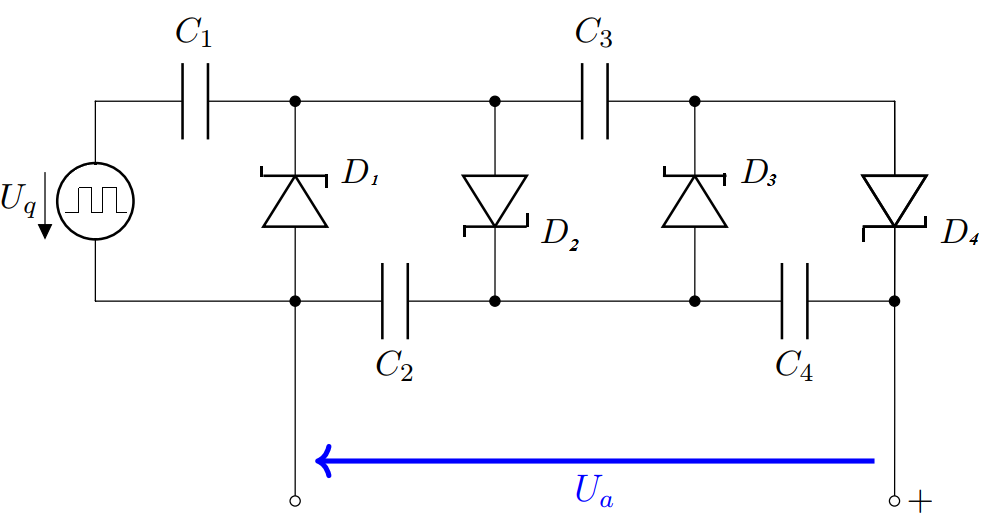
\includegraphics[width=0.8\textwidth]{schaltung}
	\captionof{figure}{4C/4D Kaskade als Vorlage zur Versuchsanordnung}
	\label{kaskadenschaltung}
\end{figure}


\laborsubsection{D}{Bilder können auch Nebeneinander}
\begin{figure}[H]
	\centering
	\begin{subfigure}[b]{0.45\textwidth} % b steht für am Boden ausrichten, damit beide captions auf gleicher Höhe
		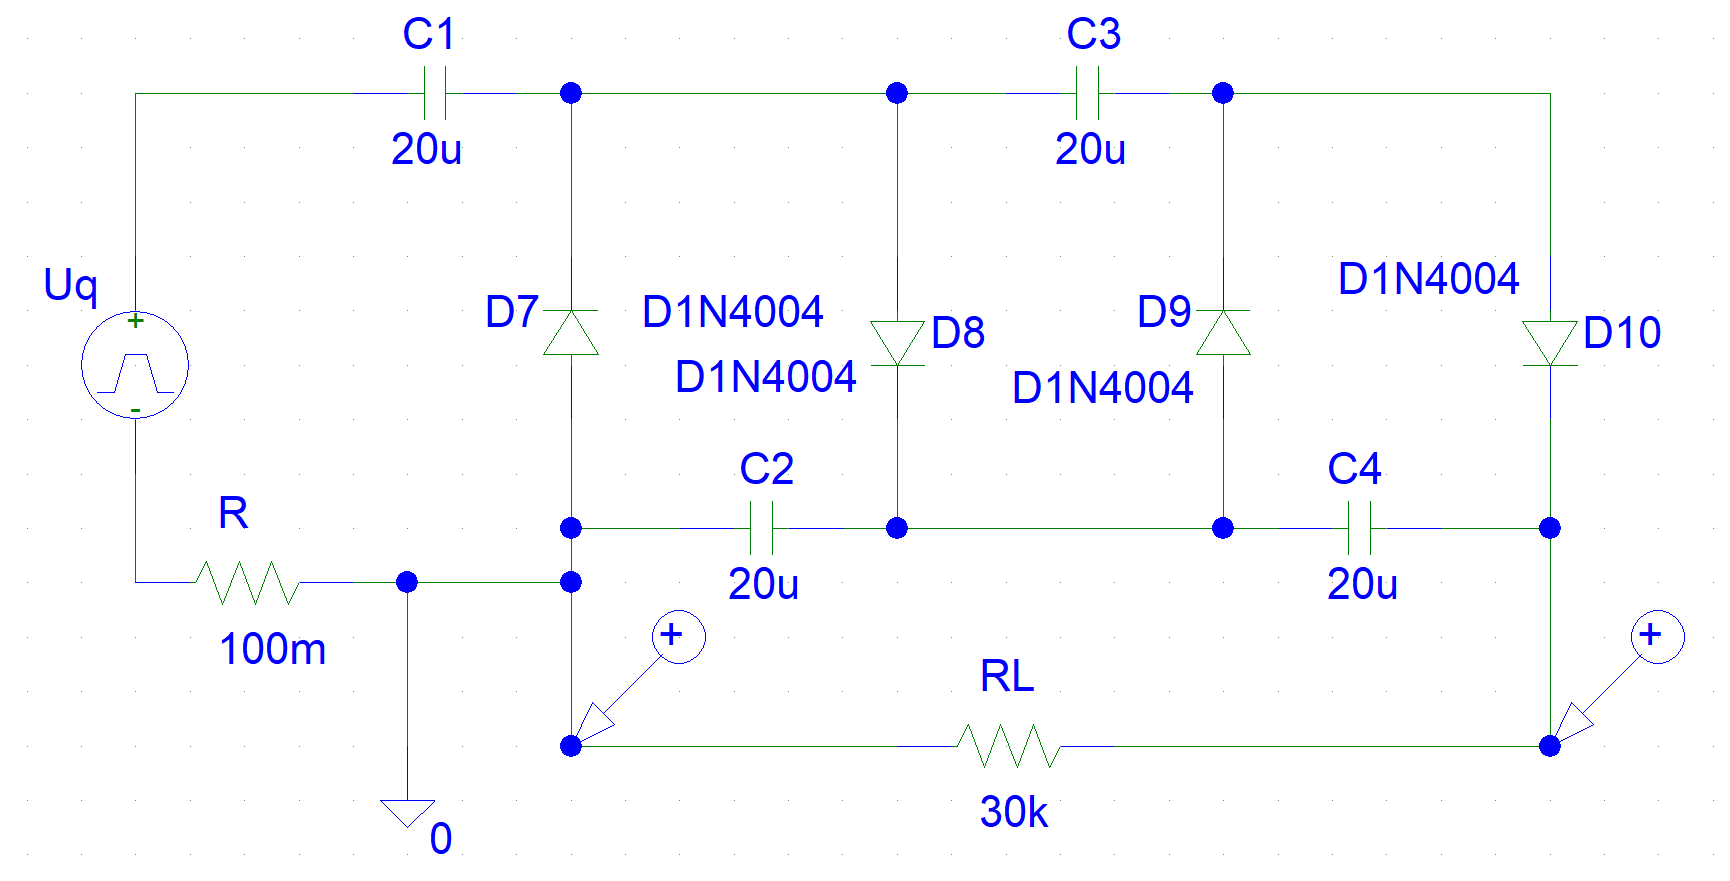
\includegraphics[width=\textwidth]{psch_kaskade}
		\subcaption{Simulation der Kaskadenschaltung (Marker für Spannungsmessung)}
		\label{psch_kaskade}
	\end{subfigure}
	\hfill % Um die beiden Figuren so weit wie möglich auseiannder zu machen
	% \hspace{0.1\textwidth} % Oder: Um einen festen Space zwischen den Figuren zu machen
	\begin{subfigure}[b]{0.45\textwidth}
		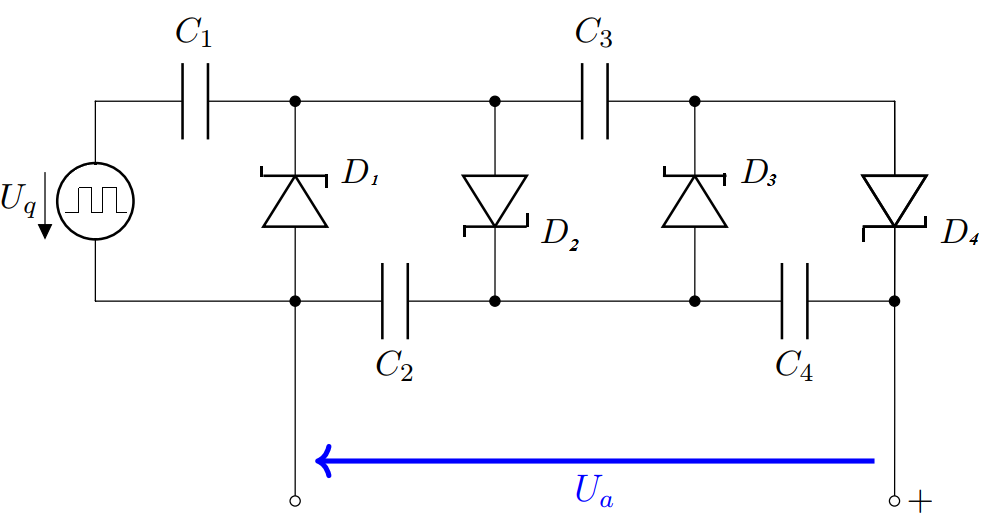
\includegraphics[width=\textwidth]{schaltung}
		\subcaption{4C/4D Kaskade als Vorlage zur Versuchsanordnung}
		\label{kaskadenschaltung_2}
	\end{subfigure}
	\caption{Gesamtdarstellung von irgendwas}
\end{figure}


\resetlaborsectioncounter
\laborsubsection{A}{Tabelle}

\begin{table}[H]
	\centering
	\renewcommand{\arraystretch}{2} % Senkrechten Abstand für diese Tabelle erhöhen
	\setlength{\tabcolsep}{0.3em} % Horizontalen Abstand für diese Tabelle erhöhen
	% S in table richtet diese nach kommata aus
	% dies funktioniert bei starkunsymetreischen zahlen nicht.
	% dazu kann man mit table-format = A.B die anzahl der erwarteten stellen eingeben dabei steht A für die Anzahl der zahlen vor dem komma und B fur die Anzahl hinter dem komma
	% test in der spalte mit {} umklammern bsp {text $P_A$}
	
	% \makecell{ 1. zeile \\ 2. zeile} ermögtlicht einfache zeilenumbrüche in einer zelle
	\begin{tabular}{|c|c|S[ table-format = 2.3]|S[ table-format = 2.3]|S[ table-format = 1.4]|S[ table-format = 1.4]|}
		\hline
		\multicolumn{2}{|c|}{}& {\makecell{Ergebnis\\ der Wirkleistung \\ aus der Simulation \\ in Watt}} & {\makecell{berechnete \\Wirkleistung\\ in Watt}} &{Abweichungen} &{\makecell{Abweichung\\ in \%}} \\ \hline
		\multirow{3}{*}{\makecell{$L_1$\\ als Bezug}} 
		&  $P_A$ & 15,500 & 15,4954 & 0,0046 & 0,0297 \\ \cline{2-6} 
		& $P_B$ & 47,761 & 47,7607 & 0,0003 & 0,0006 \\ \cline{2-6} 
		& $P_{ges}$ & 63,261 & 63,2561 & 0,0049 & 0,0077 \\ \hline
		\multirow{3}{*}{\makecell{$L_2$ \\als Bezug}}
		& $P_A$ & 38,398 & 38,3972 & 0,0008 & 0,0021 \\ \cline{2-6} 
		& $P_B$ & 24,863 & 24,8624 & 0,0006 & 0,0024 \\ \cline{2-6} 
		& $P_{ges}$ & 63,261 & 63,2596 & 0,0014 & 0,0022 \\ \hline
	\end{tabular}
\end{table}


\begin{table}[H]
	\centering
	\caption{The \texttt{s} column processes everything.}
	\label{tab:s:processing}
	\begin{tabular}{ss}
		\toprule
		{Unit} & \multicolumn{1}{c}{Unit}\\
		\midrule
		{\si{m^3}} & \multicolumn{1}{c}{\SI{}{m^3}} \\
		\kilogram & \kilogram \\
		\bottomrule
	\end{tabular}
\end{table}



	%% um seins alleine (ohne labels des anderen) zuarbeiten ein % davor weg 
% standart einstellung ist alleine arbeiten 
%!TeX root = Vorlage_nur_inhalt2.tex
% um das gesammte dokuemnt zu erstellen oder um die labels des anderen zu nutzen einmalig ein % wegmachen und nach dem man fertig ist wieder ein % zeichen davor und bei der zeile darüber ein % weg sodass %!... steht
%% !TeX root = ../Inhalt_1+2/Vorlage.tex
%a%!TEX projectfile = ../header/seiten_einstellungen.tex
%a%!TEX projectfile = header.tex
%a%!TEX projectfile = ../Inhalt2/inhalt2.tex.tex
%!TEX projectfile = ../Inhalt1/inhalt1.tex.tex

\resetlaborsectioncounter
\laborsubsection{D}{Funktion f(x) in Latex}
\begin{figure}[H]
	\centering
	\begin{tikzpicture}
		\begin{axis}[
			xlabel=Störabstand,
			ylabel=BER,
			grid=major,
			width=0.9\textwidth,
			height=0.3\textwidth]
			\addplot[color=red,mark=x] coordinates {
				(0,0.301)
				(1,0.273)
				(2,0.234)
				(3,0.185)
				(4,0.149)
				(5,0.111)
				(6,0.069)
				(7,0.04)
				(8,0.024)
			};
		\end{axis}
	\end{tikzpicture}
	\caption{Diagramm aus Koordinaten}
	\label{fig:2_2_diagramm}
\end{figure}


\newpage
\section{Programmiersprachen sämtlicher Art}
\laborsubsection{D}{Ja auch MATLAB}\label{code:matlab}
\begin{lstlisting}[language=matlab]
	syms x;
	c0 = 0;
	c1 = 1;
	c2 = 0.1;
	c3 = -0.05;
	X = 2; % X = 1;
	Y1dach = c1*X + (3/4)*c3*X^3;
	Y2dach = (1/2)*c2*X^2;
	Y3dach = (1/4)*c3*X^3;
	Y1eff = (1/sqrt(2)) * Y1dach;
	Y2eff = (1/sqrt(2)) * Y2dach;
	Y3eff = (1/sqrt(2)) * Y3dach;
	Ygeseff = sqrt(Y1eff^2 + Y2eff^2 + Y3eff^2);
	
	k2 = Y2eff/Ygeseff
	k3 = Y3eff/Ygeseff
	kges = sqrt(k2^2 + k3^2)
	
\end{lstlisting}








\newpage
\section*{Geräteliste}
\begin{table} [H]
	\label{tab:geraeteliste}
	\begin{tabular}{|l|l|}
		\hline
		\textbf{Gerät }            & \textbf{Nummer }            \\ \hline
		Multimeter Keysight U1241C & AMES\_13, AMES\_14,AMES\_15 \\ \hline
		Stelltrafo                 & 27-15                       \\ \hline
		Stelltrafo                 & 29-24                       \\ \hline
		Ringkerntrafo              & 97-24                       \\ \hline
		Digitalmultimeter          & 40-24                       \\ \hline
	\end{tabular}
\end{table}

	\printbibliography
	
\end{document}
